%%%%%%%%%%%%%%%%%%%%%%%%%%%%%%%%%%%%%%%%%%%%%%%%%%%%%%%%%%%%%%%%%%%%
% PREAMBLE
%%%%%%%%%%%%%%%%%%%%%%%%%%%%%%%%%%%%%%%%%%%%%%%%%%%%%%%%%%%%%%%%%%%%

\documentclass[handout]{beamer}
%\documentclass{beamer}

%------------------------------------------------------------------
% Presentation Settings
%------------------------------------------------------------------

\mode<presentation>
{
	\usetheme{Boadilla}      % or Boadilla, Singapore, ...
	\usecolortheme{default} % or albatross, beaver, crane, ...
	\usefonttheme{default}  % or serif, structurebold, ...
	\setbeamertemplate{navigation symbols}{}
	\setbeamertemplate{caption}[numbered]
	\setbeamertemplate{itemize items}[circle]
	\setbeamertemplate{itemize subitem}[triangle]
	\setbeamertemplate{enumerate items}[default]
	\setbeamerfont{caption}{size=\tiny}
	%\setbeamercolor{alerted text}{fg=blue}
}

%------------------------------------------------------------------
% Packages
%------------------------------------------------------------------
\usepackage{amsmath}
\usepackage[natbibapa]{apacite}
\usepackage{appendixnumberbeamer}
\usepackage[english]{babel}
\usepackage{comment}
\usepackage{hyperref}
\usepackage[utf8x]{inputenc}
\usepackage{pdfpages}
\usepackage{subcaption}
\usepackage{verbatim}

\usepackage{listings} % Code blocks
\usepackage{color}

\definecolor{ltgreen}{RGB}{230, 242, 230}

\lstset{frame=tb,
  language=bash,
  aboveskip=3mm,
  belowskip=3mm,
  showstringspaces=false,
  columns=flexible,
  basicstyle={\small\ttfamily},
  numbers=none,
  breaklines=true,
  breakatwhitespace=true,
  tabsize=3,
  backgroundcolor=\color{ltgreen}
}


%------------------------------------------------------------------
% Set up
%------------------------------------------------------------------

% Add section titles

\AtBeginSection[]{
	\begin{frame}
  	\vfill
  	\centering
  	\begin{beamercolorbox}[sep=8pt,center,shadow=false,rounded=false]{title}
    	\usebeamerfont{title}\insertsectionhead\par%
  	\end{beamercolorbox}
  	\vfill
  \end{frame}
}

% Reduce references font size

\renewcommand*{\bibfont}{\scriptsize}

%------------------------------------------------------------------
% Title page settings
%------------------------------------------------------------------

\title[Git/GitHub Workshop: Part 3]{Workshop: Introduction to Git and GitHub}

\subtitle{Part 3: Git Branching}

\author[P. Joly]{Philippe Joly}
\institute[FU-Berlin]{Freie Universität Berlin}

\date{March 9, 2021}

%%%%%%%%%%%%%%%%%%%%%%%%%%%%%%%%%%%%%%%%%%%%%%%%%%%%%%%%%%%%%%%%%%%%
% DOCUMENT
%%%%%%%%%%%%%%%%%%%%%%%%%%%%%%%%%%%%%%%%%%%%%%%%%%%%%%%%%%%%%%%%%%%%

\begin{document}

%------------------------------------------------------------------
% Title Page
%------------------------------------------------------------------
\begin{frame}
\titlepage
\end{frame}
%

%\begin{columns}
%  \begin{column}{0.5\textwidth}
%
%    ...
%
%  \end{column}
%  \begin{column}{0.5\textwidth}
%    ...
%  \end{column}
%\end{columns}

%\begin{lstlisting}
%$ cd /home/user/my_project
%\end{lstlisting}

%\begin{figure}
%	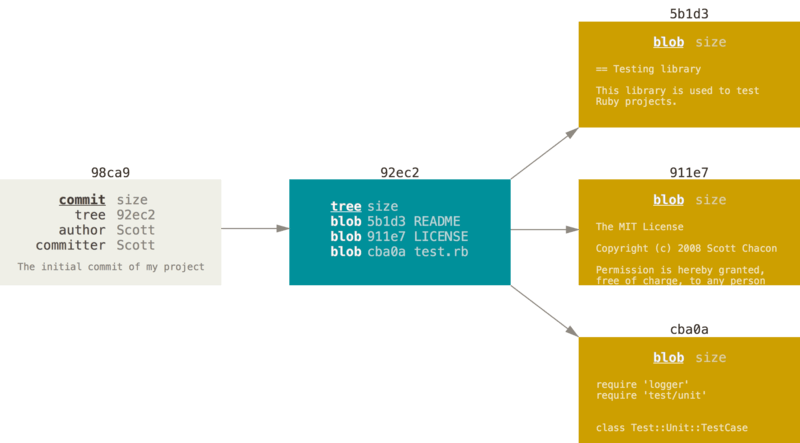
\includegraphics[width=0.9\textwidth]{figures/fig09_commit.png}
%	\caption{A commit and its tree. \textit{Source}: Chacon \& Straub (2021), fig. 9.}
%\end{figure}

%%------------------------------------------------------------------

\begin{frame}{Reference}
	\begin{columns}
	
		\begin{column}{0.5\textwidth}
			\begin{itemize}
				\item This workshop draws extensively on Scott Chacon and Ben Straub (2021), \href{https://git-scm.com/book/en/v2}{\textit{ProGit}}, Version 2.1.295, 2021-02-26. 
				\item Like the book, this workshop carries the CC BY-NC-SA 3.0 license.
			\end{itemize}
		\end{column}
		
		\begin{column}{0.5\textwidth}
			\begin{figure}
				
\includegraphics[width=0.5\textwidth]{figures/progit_cover.png}
				\caption{}
			\end{figure}
		\end{column}
	
	\end{columns}
\end{frame}

%%------------------------------------------------------------------

\section{How Git branching works}

\begin{frame}{Git branching}
	\begin{itemize}
		\item A divergence from the main line of development
		\item Git “killer feature”
		\begin{itemize}
			\item Lightweight
			\item Fast
			\item Encourages workflows that branch and merge often
			\item Let's you freely experiment
			\item Structures collaboration
		\end{itemize}
	\end{itemize}
\end{frame}
	
\begin{frame}{A branch is simply a pointer}
\begin{figure}
	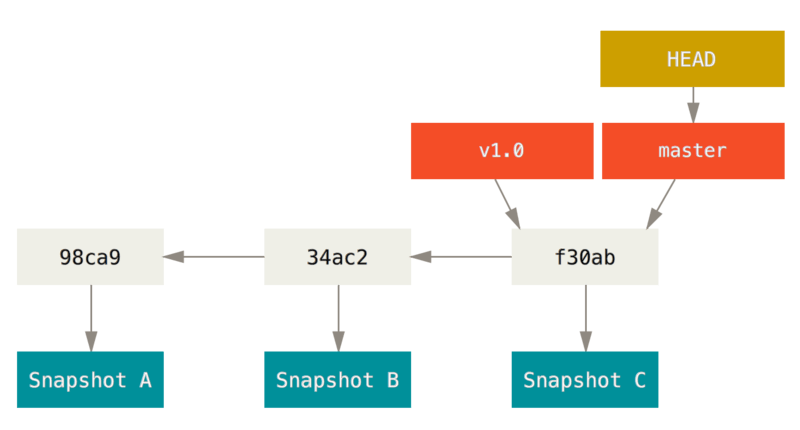
\includegraphics[width=0.9\textwidth]{figures/fig11_branch_history.png}
	\caption{A branch and its commit history. \textit{Source}: Chacon \& Straub (2021), fig. 11.}
\end{figure}
\end{frame}	

\begin{frame}[fragile]{Creating a branch adds a pointer to your commit history}
\begin{lstlisting}
$ git branch testing
\end{lstlisting}
\begin{figure}
	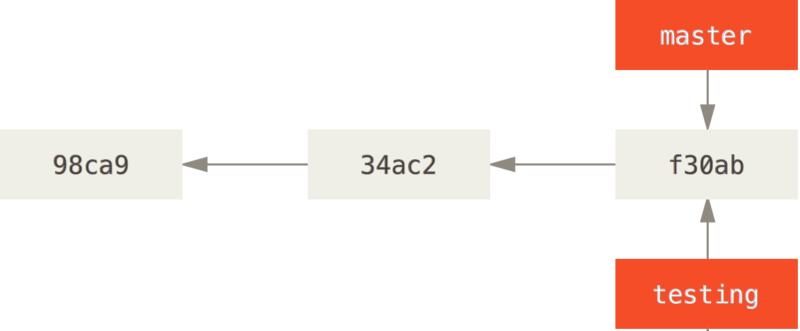
\includegraphics[width=0.9\textwidth]{figures/fig12_new_branch.png}
	\caption{Two branches pointing into the same series of commits. \textit{Source}: Chacon \& Straub (2021), fig. 12.}
\end{figure}
\end{frame}

\begin{frame}[fragile]{HEAD points to your current position}
\begin{lstlisting}
$ git branch
* master
  testing
\end{lstlisting}
\begin{figure}
	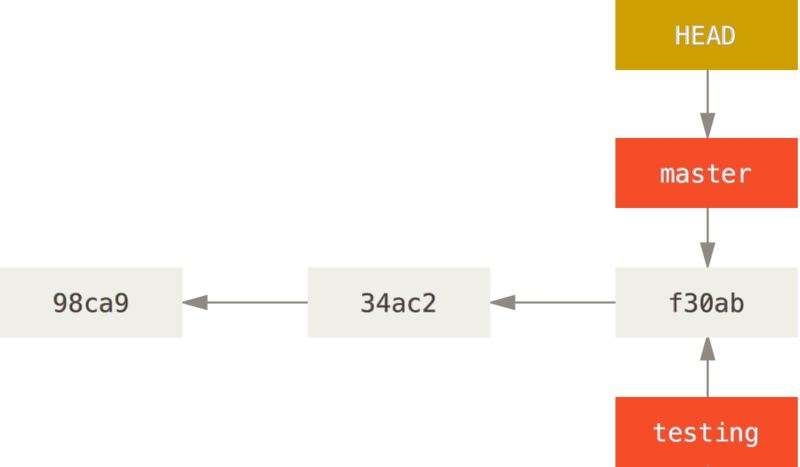
\includegraphics[width=0.8\textwidth]{figures/fig13_head.png}
	\caption{HEAD pointing to a branch. \textit{Source}: Chacon \& Straub (2021), fig. 13.}
\end{figure}
\end{frame}

\begin{frame}[fragile]{Switching branches}
\begin{lstlisting}
$ git checkout testing
$ git branch
  master
* testing
\end{lstlisting}
\begin{figure}
	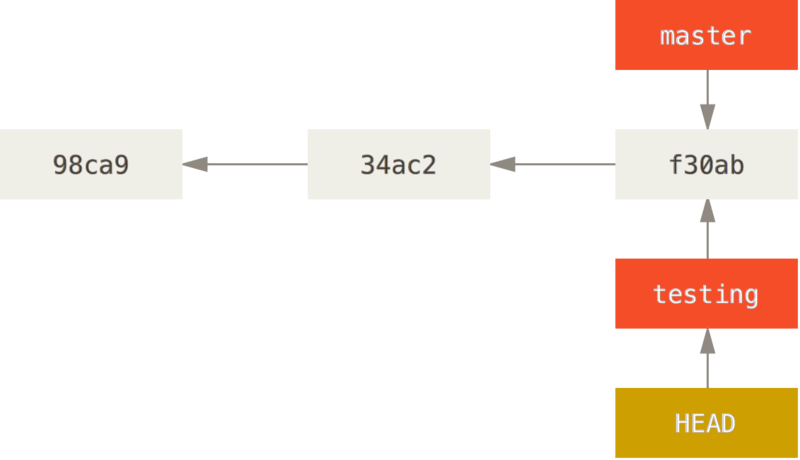
\includegraphics[width=0.7\textwidth]{figures/fig14_head_switch.png}
	\caption{HEAD points to the current branch. \textit{Source}: Chacon \& Straub (2021), fig. 14.}
\end{figure}
\end{frame}

\begin{frame}[fragile]{The new branch moves forward}

\begin{lstlisting}
$ git add myfile.txt
$ git commit -m "add this new file"
\end{lstlisting}

\begin{figure}
	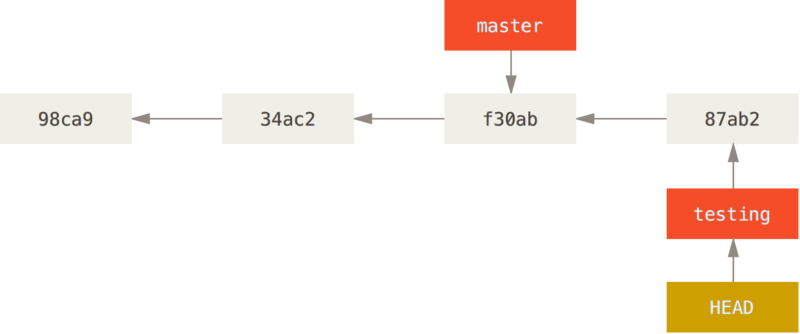
\includegraphics[width=0.9\textwidth]{figures/fig15_testing_forward.png}
	\caption{HEAD points to the current branch. \textit{Source}: Chacon \& Straub (2021), fig. 15.}
\end{figure}
\end{frame}


\begin{frame}[fragile]{Back to \texttt{master} (the main branch)}

\begin{lstlisting}
$ git checkout master
\end{lstlisting}

\begin{figure}
	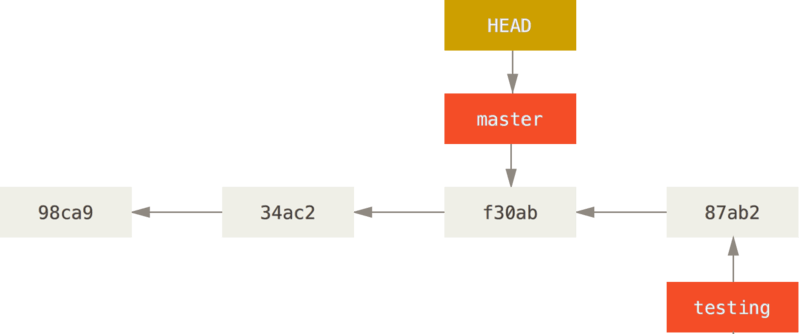
\includegraphics[width=0.9\textwidth]{figures/fig16_back_to_master.png}
	\caption{HEAD moves when you checkout. \textit{Source}: Chacon \& Straub (2021), fig. 16.}
\end{figure}
\end{frame}

\begin{frame}[fragile]{\texttt{master} moves forward: a divergent history}

\begin{lstlisting}
$ git add myfile2.txt
$ git commit -m "add another file"
\end{lstlisting}

\begin{figure}
	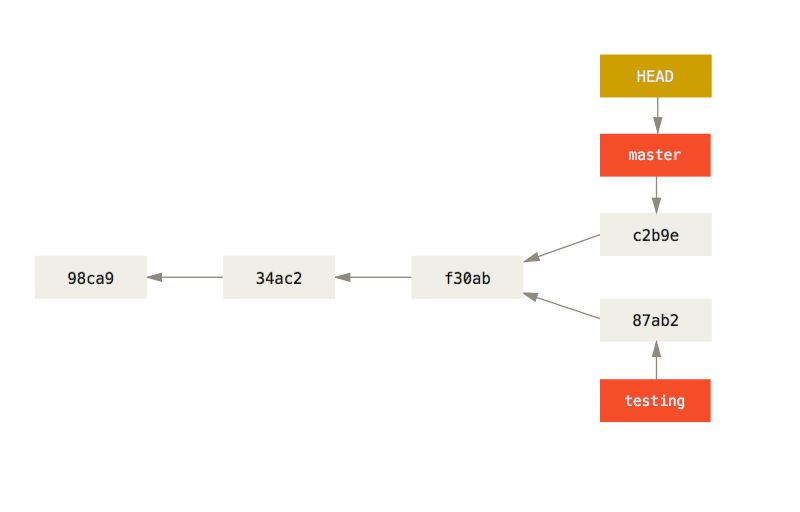
\includegraphics[width=0.7\textwidth]{figures/fig17_diverge.png}
	\caption{Divergent history. \textit{Source}: Chacon \& Straub (2021), fig. 17.}
\end{figure}
\end{frame}

\begin{frame}[fragile]{Creating and switching branches: summary}
Create a new branch
\begin{lstlisting}
$ git branch newbranch
\end{lstlisting}
Switch to that branch
\begin{lstlisting}
$ git checkout newbranch
\end{lstlisting}
Shortcut: create \textit{and} switch to a new branch 
\begin{lstlisting}
$ git checkout -b newbranch
\end{lstlisting}
List your branches and see on which one you are now
\begin{lstlisting}
$ git branch
\end{lstlisting}
\end{frame}

\section{Merging}

\begin{frame}{Basic merging (1)}
\begin{figure}
	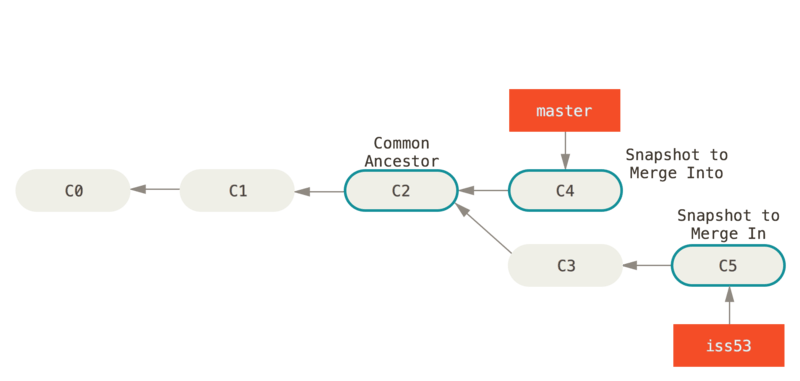
\includegraphics[width=0.9\textwidth]{figures/fig24_pre_merge.png}
	\caption{Three snapshots used in a typical merge. \textit{Source}: Chacon \& Straub (2021), fig. 24.}
\end{figure}
\end{frame}

\begin{frame}[fragile]{Basic merging (2)}
Move (\texttt{checkout}) to the \textbf{receiving} branch ({master}) before merging
\begin{lstlisting}
$ git checkout master
$ git merge iss53
\end{lstlisting}
\begin{figure}
	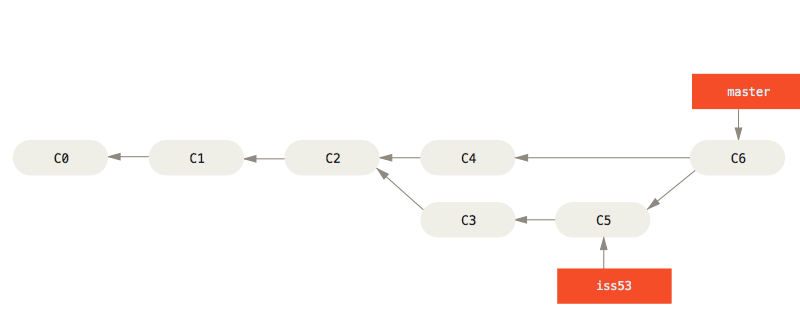
\includegraphics[width=0.9\textwidth]{figures/fig25_merge.png}
	\caption{A merge commit. \textit{Source}: Chacon \& Straub (2021), fig. 25.}
\end{figure}
\end{frame}

\begin{frame}[fragile]{Deleting a branch}
After merging, you can safely delete the branch. 
\begin{lstlisting}
$ git branch -d iss53
\end{lstlisting}
\end{frame}

\section{Merge Conflicts}

\begin{frame}[fragile]{Basic Merge Conflicts (1)}

If you have modified the same lines, of the same file, in both branches, you will have a merge conflict. 

\begin{lstlisting}
$ git merge iss53
Auto-merging index.html
CONFLICT (content): Merge conflict in index.html
Automatic merge failed; fix conflicts and then commit the result.
\end{lstlisting}

\end{frame}

\begin{frame}[fragile]{Basic Merge Conflicts (2)}

Git handles this problem by inserting markers in your file to highlight the merge conflict.

\begin{lstlisting}
<<<<<<< HEAD:index.html
<div id="footer">contact : email.support@github.com</div>
=======
<div id="footer">
 please contact us at support@github.com
</div>
>>>>>>> iss53:index.html
\end{lstlisting}

\end{frame}

\begin{frame}{Basic Merge Conflicts (3)}

Workflow:
\begin{enumerate}
	\item Open the problematic file
	\item Look for the \texttt{<<<<<<<}, \texttt{=======}, and \texttt{>>>>>>>} markers
	\item Revise this part of the file: select one of the two options or create a new one.
	\item Delete the markers. 
	\item Save your file.
	\item Stage your changes using \texttt{git add}.
	\item Finalize your merge using \texttt{git commit}.
\end{enumerate}

\end{frame}

\begin{frame}[fragile]{Inspect your merging history}

\begin{lstlisting}
$ git log --oneline --graph --all

*   c545382 (HEAD -> main) Manage the merge conflict
|\  
| * a6afe91 Modify the same lines on newbranch
* | e621ec9 Change something on main
|/  
* 764a766 Initial commit
\end{lstlisting}

\end{frame}


\section{Exercise}

\begin{frame}[fragile]{Exercise 1 (a)}

1. Open a new folder and initialize a new repo.
\begin{lstlisting}
$ git init 
\end{lstlisting}
2. Create a file named \texttt{list.md} with a list of \textbf{three places} you would like to visit after the pandemic.

\vspace{0.3cm}

3. Stage and commit your changes.

\begin{lstlisting}
$ git add list.md
$ git commit list.md
\end{lstlisting}

\end{frame}

\begin{frame}[fragile]{Exercise 1 (b)}

4. Create and switch to a new branch
\begin{lstlisting}
$ git checkout -b newbranch
\end{lstlisting}

5. Modify the third item on your list.

\vspace{0.3cm}

6. Stage and commit your changes.

\begin{lstlisting}
$ git add list.md
$ git commit list.md
\end{lstlisting}

7. Switch back to the main branch
\begin{lstlisting}
$ git checkout main
\end{lstlisting}

8. Repeat steps 5 and 6 but modify the third item differently this time. 

\end{frame}

\begin{frame}[fragile]{Exercise 1 (c)}



\vspace{0.3cm}

9. Try merging

\begin{lstlisting}
$ git merge newbranch
\end{lstlisting}

10. Open \texttt{list.md} and manage the merge conflict

\vspace{0.3cm}

11. Stage and finalize your merge

\begin{lstlisting}
$ git add list.md
$ git commit list.md
\end{lstlisting}

12. Inspect your merging history

\begin{lstlisting}
$ git log --oneline --graph --all
\end{lstlisting}

13. Delete \texttt{newbranch}

\begin{lstlisting}
$ git branch -d newbranch
\end{lstlisting}

\end{frame}

\section{Workflows}

\begin{frame}{Git Feature Branch Workflow}
\begin{figure}
	
\includegraphics[width=0.9\textwidth]{figures/feature_branch.pdf}
	\caption{Feature Branch Workflow. \textit{License}: CC BY 2.5 AU. \textit{Source}: Atlassian. \href{https://www.atlassian.com/git/tutorials/comparing-workflows/feature-branch-workflow}{https://www.atlassian.com}}
\end{figure}
\begin{itemize}
	\item All feature development takes place in a dedicated branch.
	\item The main branch should not contain broken code.
	\item Merges are the focal point of discussion in a team.
\end{itemize}
\end{frame}

\begin{frame}{Gitflow for more complex projects}
\begin{figure}
	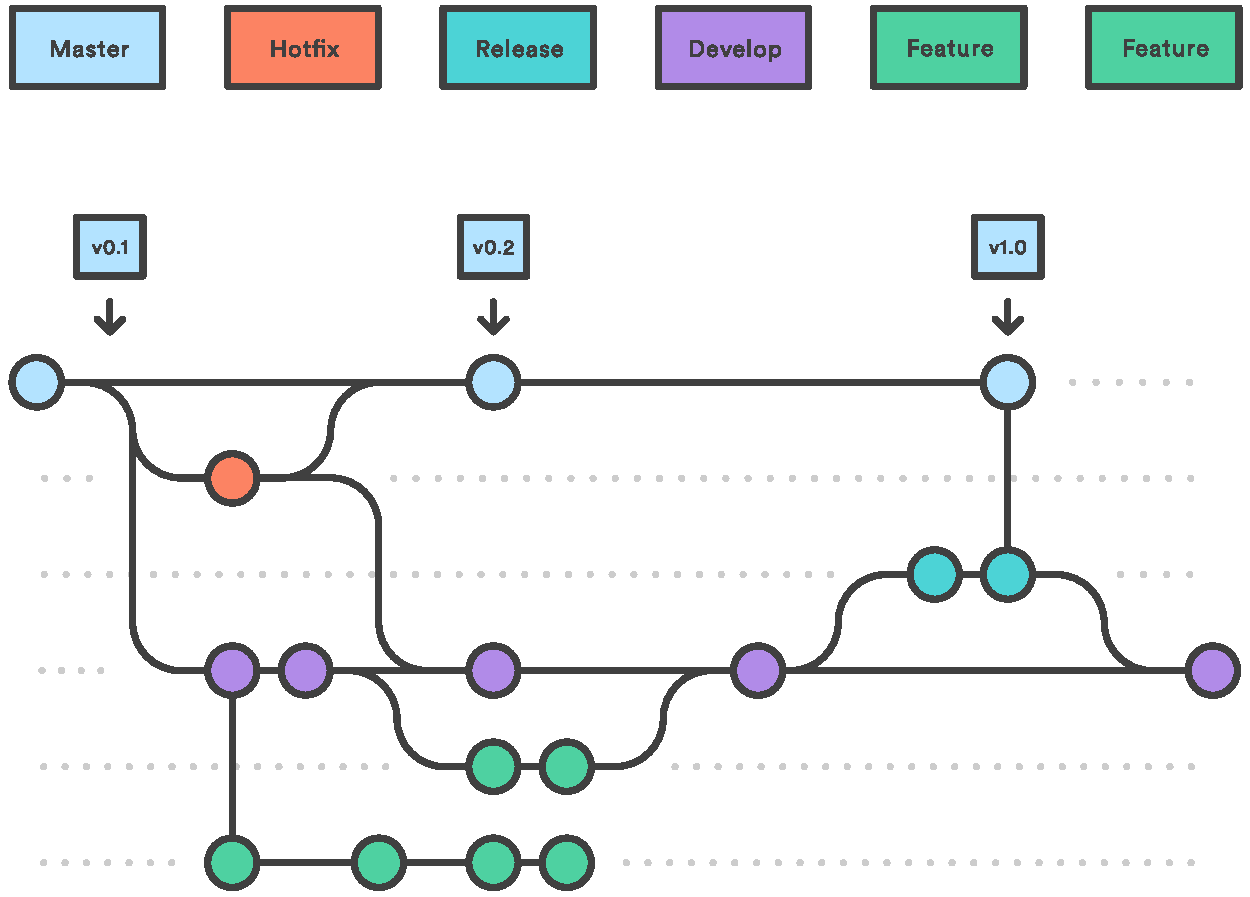
\includegraphics[width=0.8\textwidth]{figures/gitflow.pdf}
	\caption{Gitflow. \textit{License}: CC BY 2.5 AU. \textit{Source}: Atlassian. \href{https://www.atlassian.com/git/tutorials/comparing-workflows/gitflow-workflow}{https://www.atlassian.com}}
\end{figure}
\end{frame}

\section{Refresher: working with remotes}

\begin{frame}{Refresher: working with remotes (1)}
\begin{figure}
	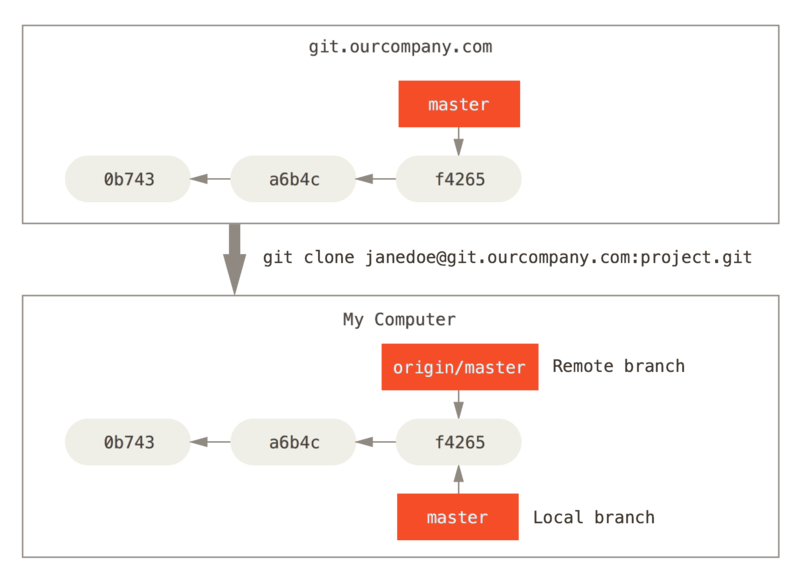
\includegraphics[width=0.8\textwidth]{figures/fig30_clone.png}
	\caption{Server and local repositories after cloning. \textit{Source}: Atlassian. Chacon \& Straub, fig. 30.}
\end{figure}
\end{frame}

\begin{frame}{Refresher: working with remotes (2)}
\begin{figure}
	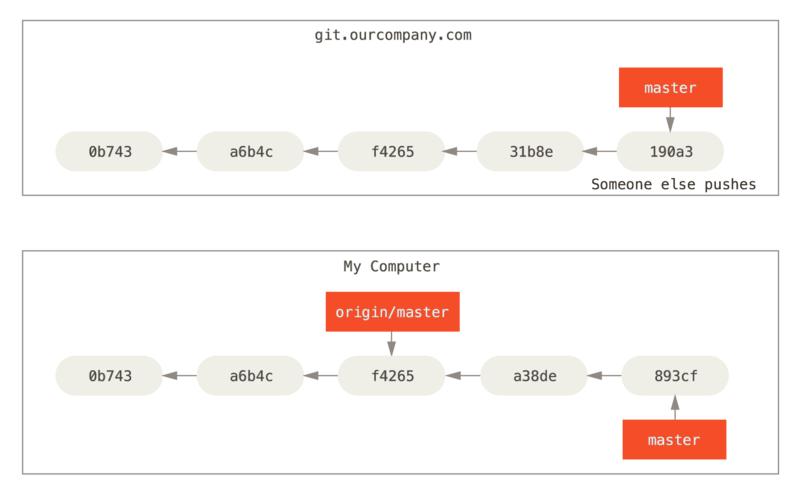
\includegraphics[width=0.8\textwidth]{figures/fig31_local_forward.png}
	\caption{Local and remote work can diverge. \textit{Source}: Atlassian. Chacon \& Straub, fig. 31.}
\end{figure}
\end{frame}

\begin{frame}{Refresher: working with remotes (3)}
\begin{figure}
	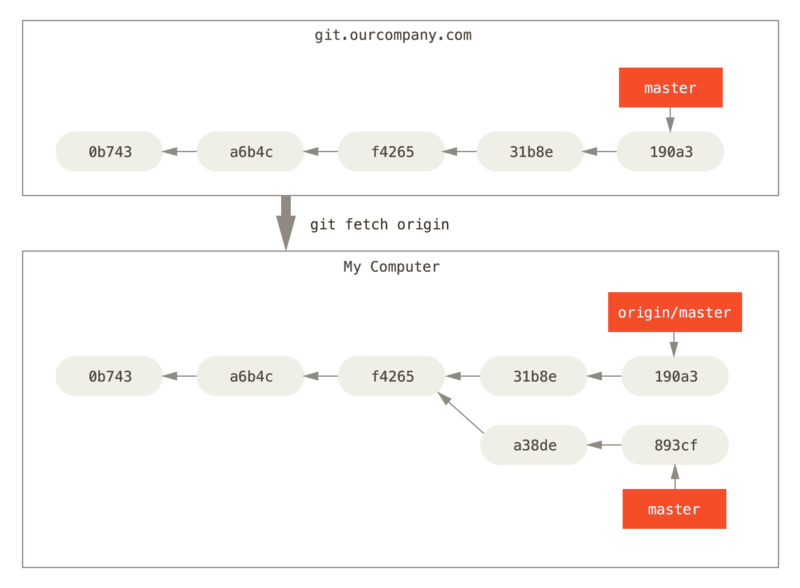
\includegraphics[width=0.8\textwidth]{figures/fig32_diverge.png}
	\caption{\texttt{git fetch} updates your remote-tracking branches. \textit{Source}: Atlassian. Chacon \& Straub, fig. 32.}
\end{figure}
\end{frame}

\begin{frame}[fragile]{Refresher: working with remotes (4)}
Update the version history of the server on your computer:
\begin{lstlisting}
$ git fetch origin
\end{lstlisting}
Examine the differences between your local branch and the branch on the server:
\begin{lstlisting}
$ git diff origin/main
\end{lstlisting}
If needed, merge:
\begin{lstlisting}
$ git merge origin/main
\end{lstlisting}

\end{frame}

\begin{frame}{\texttt{git pull}}
\begin{itemize}
	\item \texttt{git pull} is a \textbf{shortcut} for \texttt{git fetch} and \texttt{git merge}.
	\item This command is \alert{dangerous} because it can overwrite your working directory without giving you the chance to examine the changes. 
	\item It's usually better to run \texttt{git fetch}, examine the changes with \texttt{git diff}, and then run \texttt{git merge}.
\end{itemize}
\end{frame}

\section{Exercise}

\begin{frame}[fragile]{Exercise 2}

1. Log into GitHub and open the demo repository you created in Exercise 3 of Part 2 of the workshop. 

\vspace{0.3cm}

2. Modify \texttt{README.md} and commit your changes \textbf{online}. 

\vspace{0.3cm}

3. In your \textbf{local} repo, update the version history of the server.

\begin{lstlisting}
$ git fetch origin
\end{lstlisting}

4. Examine the differences between your local version history and the version history on the server. 

\begin{lstlisting}
$ git status
$ git diff origin/main
\end{lstlisting}

5. Merge the version history of the server into your local main branch.

\begin{lstlisting}
$ git merge origin/main
\end{lstlisting}
\end{frame}

\section{Remote branches}

\begin{frame}[fragile]{Working with remote branches (1)}{Scenario 1: Create a new branch and share it on a remote}

Create and switch to a new branch:

\begin{lstlisting}
$ git checkout -b newbranch
\end{lstlisting}

Push this branch to the remote: 

\begin{lstlisting}
$ git push origin newbranch
\end{lstlisting}

Start tracking the remote branch:

\begin{lstlisting}
$ git branch -u origin/newbranch
\end{lstlisting}

In other words, when you \texttt{git push} and \texttt{git fetch}, Git will automatically compare your local \textbf{tracking branch} with the \textbf{remote upstream} branch. 

\end{frame}

\begin{frame}[fragile]{Working with remote branches (2)}{Inspect your tracking and upstream branches}

\begin{lstlisting}
$ git branch -vv
  main       d2abadb [origin/main] Update README.md
* newbranch d2abadb [origin/newbranch] Update README.md
\end{lstlisting}

\begin{itemize}
	\item The local \texttt{main} branch is tracking the upstream \texttt{main} branch on the remote \texttt{origin}.
	\item The local \texttt{newbranch} is tracking the upstream \texttt{newbranch} on the remote \texttt{origin}.
\end{itemize} 

\end{frame}


\begin{frame}[fragile]{Working with remote branches (3)}{Scenario 2: Import a branch created by someone else on the remote}

Fetch the remote repository. Git informs you about the new branch: 

\begin{lstlisting}
$ git fetch
From github.com:jolyphil/demorepo
 * [new branch]      newbranch        -> origin/newbranch

\end{lstlisting}

\texttt{newbranch} is still not a local branch:

\begin{lstlisting}
$ git branch
* main
\end{lstlisting}

Create a local copy and switch to it: 

\begin{lstlisting}
$ git checkout --track origin/newbranch
Branch 'newbranch' set up to track remote branch 'newbranch' from 'origin'.
Switched to a new branch 'newbranch'
\end{lstlisting}

\end{frame}

\begin{frame}[fragile]{Deleting a remote branch}

Switch back to \texttt{main}:

\begin{lstlisting}
$ git checkout main
\end{lstlisting}

Delete the local branch:

\begin{lstlisting}
$ git branch -d mybranch
\end{lstlisting}

Delete the remote branch:

\begin{lstlisting}
$ git push origin --delete mybranch
\end{lstlisting}

\end{frame}


\section{Exercise}

\begin{frame}[fragile]{Exercise 3}

1. Open the repo used in the previous exercise. 

\vspace{0.3cm}

2. Create and switch to a new branch named 'newfeature'.

\begin{lstlisting}
$ git checkout -b newfeature
\end{lstlisting}

3. Push this branch to the remote.

\begin{lstlisting}
$ git push origin newfeature
\end{lstlisting}

4. Start tracking the remote branch.

\begin{lstlisting}
$ git branch -u origin/newfeature
\end{lstlisting}

5. Inspect your tracking and upstream branches.

\begin{lstlisting}
$ git branch -vv
\end{lstlisting}

\end{frame}

\end{document}

